% Slides for 2025-07-01
%To create a slide, use the following:
% --- SLIDE 1 ---
\begin{frame}
    \frametitle{Vector Database}
    \begin{itemize}
        \item Our JSON database is becoming too large.
        \item Search performance is slowing down.
        \item We need a more efficient solution.
    \end{itemize}
    \vspace{0.5cm}
    \centering
    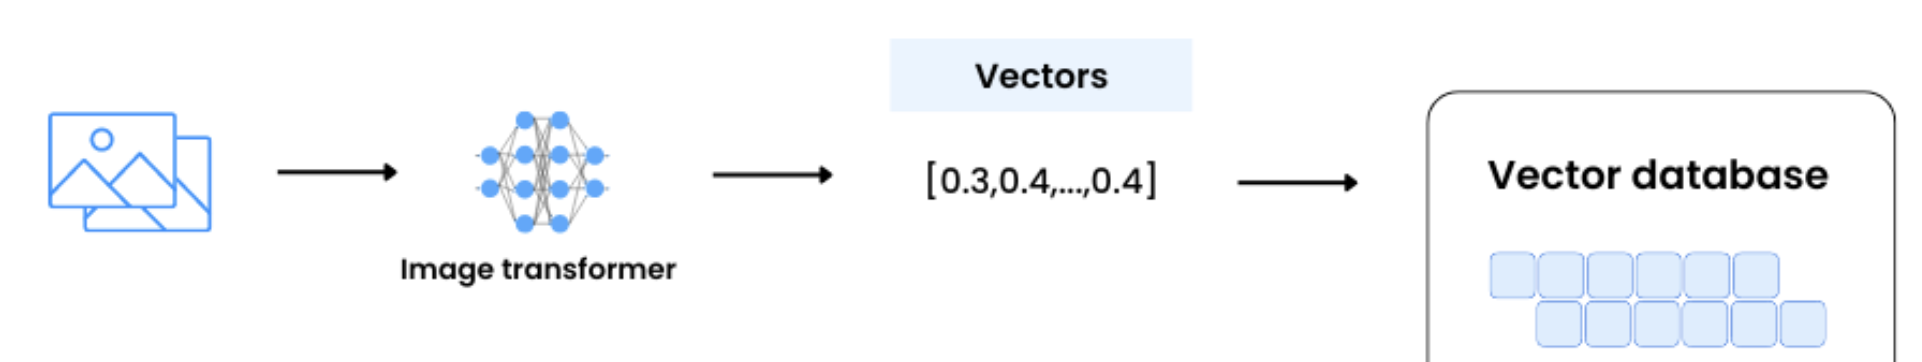
\includegraphics[width=0.8\textwidth, keepaspectratio]{images/Vectordb.png}
\end{frame}

\begin{frame}
    \frametitle{The Solution}
    \begin{itemize}
        \item Use an embedded vector database.
        \item No external server required for processing.
        \item Enables instant, efficient search results.
    \end{itemize}
\end{frame}

\begin{frame}
    \frametitle{LanceDB}
    \begin{itemize}
        \item Simple and efficient data retrieval.
        \item Fully embedded within the application.
    \end{itemize}
    \vspace{0.5cm}
    \centering
    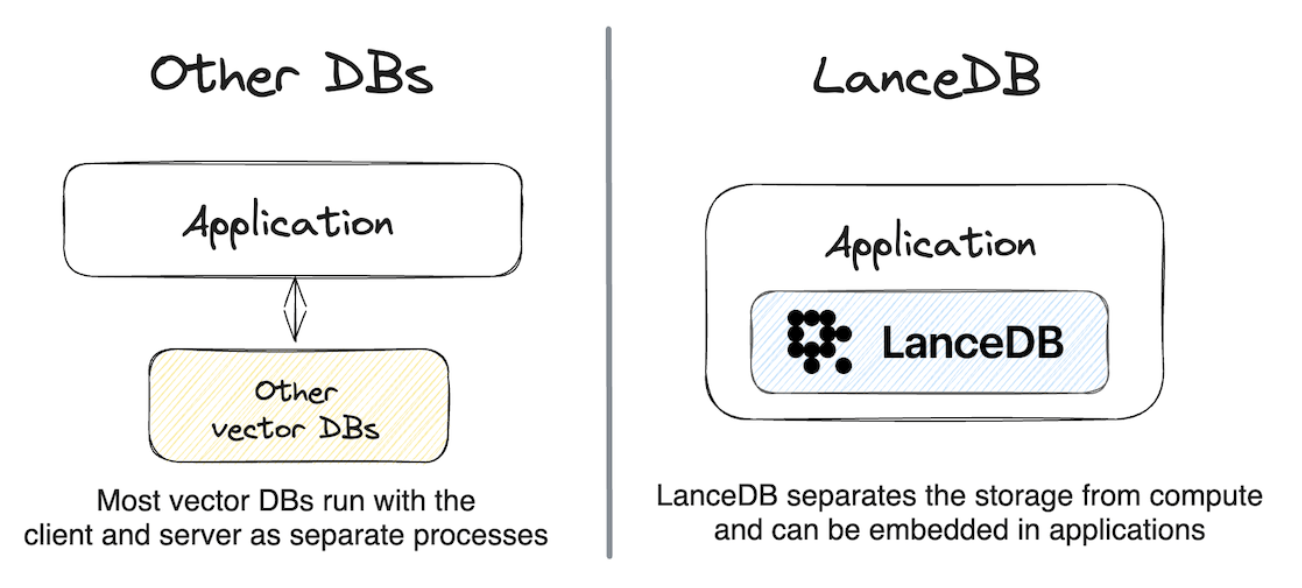
\includegraphics[width=0.8\textwidth, keepaspectratio]{images/vdbdiffernce.png}
\end{frame}

\begin{frame}
    \frametitle{Depthwise Color Consistency}
    \begin{columns}
        \begin{column}{0.5\textwidth}
            \begin{figure}
                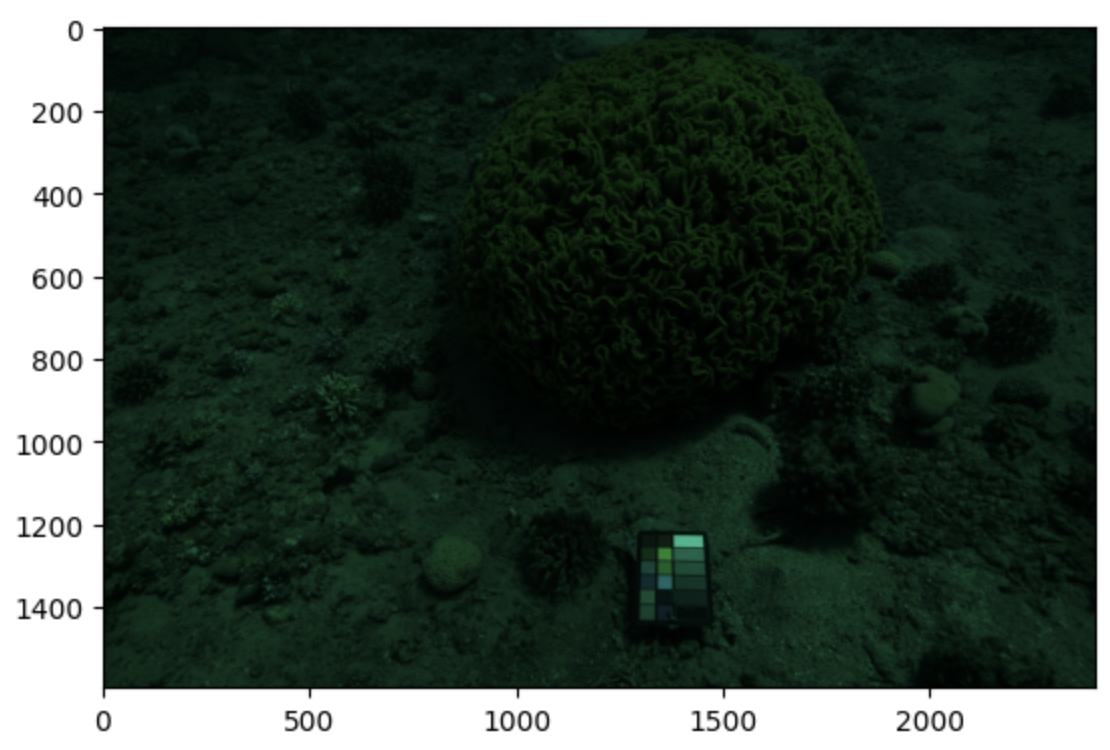
\includegraphics[width=\linewidth]{images/depth_color_issue.png}
            \end{figure}
        \end{column}    
    \end{columns}
    \begin{itemize}
        \item As depth varies, color information is lost.
        \item This makes it difficult to segment objects accurately.
    \end{itemize}
\end{frame}

\begin{frame}
    \frametitle{Our Solution: Depth-Aware Adaptive Convolution}
    \begin{columns}
        \begin{column}{0.4\textwidth}
            \begin{figure}
                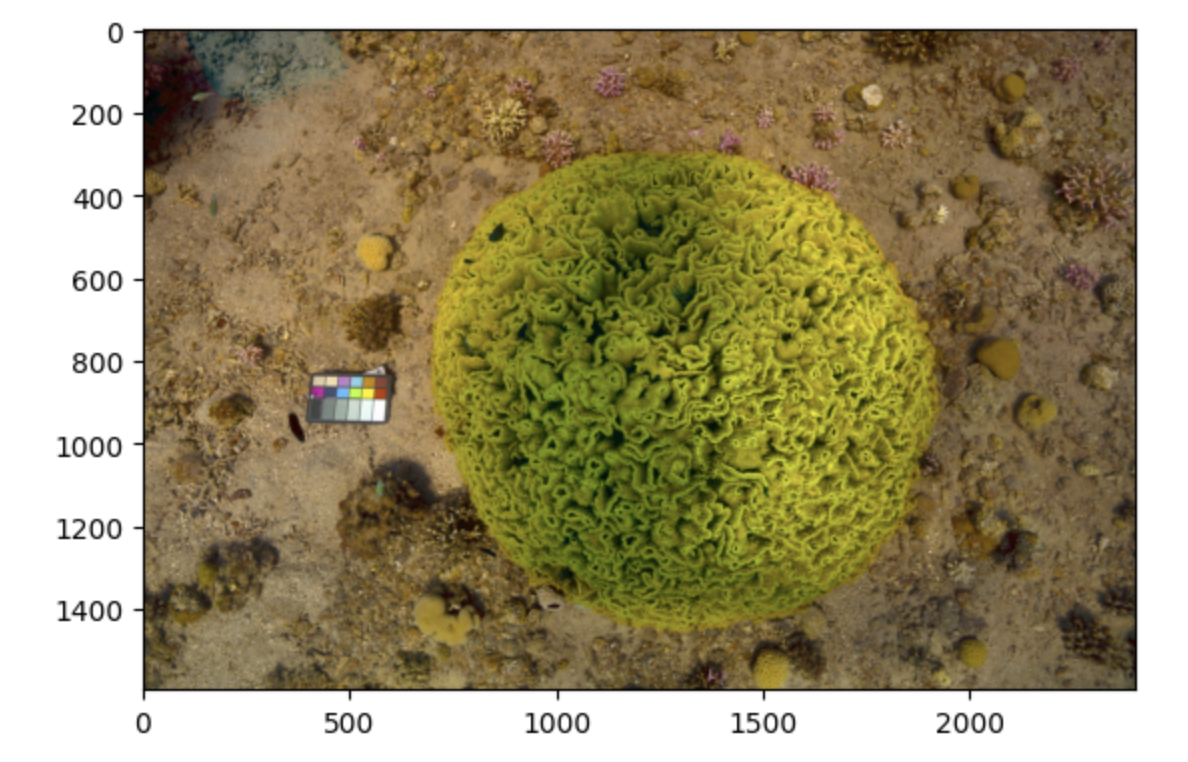
\includegraphics[width=\linewidth]{images/depth_color_corrected.png}
            \end{figure}
        \end{column}
        \begin{column}{0.6\textwidth}
            \textbf{Key Concepts:}
            \begin{itemize}
                \item Adaptive, non-fixed convolution filter.
                \item Adapts per-pixel/kernel using neighbors and depth.
                \item Enables non-uniform color correction across the image.
            \end{itemize}
        \end{column}
    \end{columns}
\end{frame}

\begin{frame}
        \frametitle{Depth-Aware Adaptive Convolution}   
    \textbf{Implementation:}
    \begin{itemize}
        \item CUDA: High-performance, parallel processing on GPUs.
        \item wgpu: Broad hardware support with Metal, Vulkan.
    \end{itemize}
\end{frame}

% To create a slide with a bullet list, use the following:
% \begin{frame}{TITLE}
%     \begin{itemize}
%         \item ITEM 1
%         \item ITEM 2
%     \end{itemize}    
% \end{frame}

% To create a slide with numbered list, use the following:
% \begin{frame}{TITLE}
%     \begin{enumerate}
%         \item ITEM 1
%         \item ITEM 2
%     \end{enumerate}
% \end{frame}

% To create a slide with a graphic:
% 1. Add the graphic to this folder (named picture.png)
% 2. Use the following:
% \begin{frame}{TITLE}
%     \centering
%     \includegraphics[height=0.7\textheight,width=0.7\textwidth,keepaspectratio]{picture.png}
% \end{frame}

% To create a slide with two columns, use the following:
% \begin{frame}{TITLE}
%     \begin{columns}
%         \begin{column}{0.5\textwidth}
%             COLUMN 1 BODY
%         \end{column}
%         \begin{column}{0.5\textwidth}
%             COLUMN 2 BODY
%         \end{column}
%     \end{columns}
% \end{frame}
